%%%%%%%%%%%%%%%%%%%%%%%%%%%%%%%%%%%%%%%%%
%
% STOKES' THEOREM
%
%%%%%%%%%%%%%%%%%%%%%%%%%%%%%%%%%%%%%%%%%
\chapter{Stokes' Theorem}

When discussing differential forms an equation called \emph{Green's Theorem} was shown. 
Green's Theorem allows for one to convert between an integral over a 2-dimensional region and a 1-dimensional integral
over a curve that bounds it.
This turns out to be just one instance of the more general \emph{Stokes' Theorem} 
which will work in higher dimensions as well.
To do so we will first need to generalize the notion of a bounding region or boundary.




%%%%%%%%%%%%%%%%%%%%%%%%%%%%%%%%%%%%%%%%%
% BOUNDARY
%%%%%%%%%%%%%%%%%%%%%%%%%%%%%%%%%%%%%%%%%
\section{Boundary Operator}


In one dimension, the boundary of an interval was quite straight-forward.
For a positively oriented interval, the boundary was composed of two points; 
the right end-point was positive and the left end-point was negative.
From the perspective of $k$-rectangles, 
the $\partial$ operator has mapped an oriented 1-rectangle to a set of oriented 0-rectangles.
We will now generalize the boundary to map an oriented $n$-rectangle to an $(n-1)$-rectangle.


\begin{definition}
	Let  $[\![\boldsymbol{a}, \boldsymbol{b}]\!]$ be a a $k$-rectangle in $\mathbb{R}^n$.
	Additionally, let $i_1, i_2, \ldots, i_k$ be the unique non-decreasing sequence of indices such that $a_{i_j} \neq b_{i_j}$.
	The \textbf{boundary of $ \boldsymbol{[\![ a,b ]\!]} $ }, denoted the operator $\partial$ is given by
	\begin{align}
		\label{eqn:defboundary}
		\partial \left( [\![ \boldsymbol{a}, \boldsymbol{b} ]\!] \right) 
		= \bigoplus_{j=1}^k (-1)^j \;
			\left(	
				[\![ 	(\boldsymbol{a}^{[\![1,n]\!]}), 
					\;\;\;
					(\boldsymbol{b}^{[\![1,i_j)\!)} 
						\oplus \boldsymbol{a}^{\hset{i_j}}
						\oplus \boldsymbol{b}^{(\!(i_j,n]\!]}) 
				]\!] \right.\;
			\notag\\
			\ominus \left.
				[\![ 	(\boldsymbol{a}^{[\![1,i_j)\!)}
						\oplus \boldsymbol{b}^{\hset{i_j}}
						\oplus \boldsymbol{a}^{(\!(i_j, n]\!]}), 
					\;\;\;		 
					(\boldsymbol{b}^{[\![1,i_j)\!)}) 			
				]\!]
			\right)
	\end{align}
\end{definition}


The above equation will require a bit of unpacking to digest featuring oriented intervals in two different contexts.
The first appears in the superscripts of $\boldsymbol{a}$ and $\boldsymbol{b}$. 
The intervals $[\![1, i_j)\!)$ and $(\!(i_j, n]\!]$ are  and is an interval over vector indices just as in Chapter 3.
Thus, the term $\boldsymbol{a}^{[\![1,i_j)\!)}$ refers to the vector $(a_1, a_2, \ldots, a_{i_j-1})$ 
while the term $\boldsymbol{b}^{(\!(i_j,n]\!]}$ refers to $(b_{i_j+1}, b_{i_j+2}, \ldots, b_{n})$.
This provides a compact notation to partition the original range of indices into 3 pieces: $[\![ 1,i_j )\!)$, $\hset{i_j}$, and $(\!(i_j, n]\!]$.
Formally, we are actually using the hybrid sets $\hset{(i_j)^1}$ but we omit multiplicity of one.


Next we use the pointwise sum $\oplus$ we reconstruct $n$-dimensional vectors from our pieces.
We then construct a $(k-1)$-rectangle using these vectors as in (\ref{eqn:defboundary}).
Hence we will have terms of the forms:
\begin{equation*}
	[\![a_1, b_1]\!]
	\times \ldots \times
	[\![a_{i_{j-1}}, b_{i_{j-1}}]\!]
	\times
	[\![a_{i_j}, a_{i_j}]\!]
	\times
	[\![a_{i_{j-1}}, b_{i_{j-1}}]\!]
	\times \ldots \times
	[\![a_n, b_n]\!]
\end{equation*}
and
\begin{equation*}
	[\![a_1, b_1]\!]
	\times \ldots \times
	[\![a_{i_{j-1}}, b_{i_{j-1}}]\!]
	\times
	[\![b_{i_j}, b_{i_j}]\!]
	\times
	[\![a_{i_{j-1}}, b_{i_{j-1}}]\!]
	\times \ldots \times
	[\![a_n, b_n]\!]
\end{equation*}


In each Cartesian product, the terms at $i_j$: $[\![a_{i_j}, a_{i_j}]\!]$ and $[\![b_{i_j}, b_{i_j}]\!]$ are both 0-cubes.
Since we defined the sequence $i_j$ by $a_{i_j} \neq b_{i_j}$, 
these 0-rectangles are replacing 1-cubes in $[\![\boldsymbol{a}, \boldsymbol{b}]\!]$.
Hence we are indeed left with a $(k-1)$-cube.




%%%%%%%%%%%%%%%%%%%%%%%%%%%%%%%%%%%%%%%%%
% BOUNDARY OF A 1-RECTANGLE
%%%%%%%%%%%%%%%%%%%%%%%%%%%%%%%%%%%%%%%%%
\subsection{Example: \emph{Boundary of a 1-rectangle}}
Let $\boldsymbol{a}= (a_1)$ and $\boldsymbol{b} = (b_1)$ be trivial 1-tuples. 
Then $[\![\boldsymbol{a}, \boldsymbol{b}]\!] = [\![a_1, b_1]\!]$
It follows that:
\begin{align*}
	\partial ( \; [\![ \boldsymbol{a}, \boldsymbol{b} ]\!] \; )
	=& \; (-1)^i ( [\![\boldsymbol{a}^{[\![1,1)\!)}, \boldsymbol{b}^{[\![1,1)\!)} ]\!]
	\times \hset{a_1} \times
	[\![\boldsymbol{a}^{(\!(1,1]\!]}, \boldsymbol{b}^{(\!(1,1]\!]} ]\!]\\
	&\; \ominus
	[\![\boldsymbol{a}^{[\![1,1)\!)}, \boldsymbol{b}^{[\![1,1)\!)} ]\!]
	\times \hset{b_1} \times
	[\![\boldsymbol{a}^{(\!(1,1]\!]}, \boldsymbol{b}^{(\!(1,1]\!]} ]\!] )\\
	=& \; \ominus [\![\boldsymbol{a}^{\emptyset}, \boldsymbol{b}^{\emptyset} ]\!]
	\times \hset{a_1} \times
	[\![\boldsymbol{a}^{\emptyset}, \boldsymbol{b}^{\emptyset} ]\!]
	\oplus
	[\![\boldsymbol{a}^{\emptyset}, \boldsymbol{b}^{\emptyset} ]\!]
	\times \hset{b_1} \times
	[\![\boldsymbol{a}^{\emptyset}, \boldsymbol{b}^{\emptyset} ]\!] \\
	=& \; \hset{a^{-1}, b^{1}}
\end{align*}

One may notice the similarity between this result and the (second) fundamental theorem of calculus:
\begin{equation*}
	\int_a^b F'(x) \; \diff x = F(b) - F(a)
\end{equation*}
Which one could easily rewrite as $\int_{[\![a,b]\!]} F'(x) \; \diff x = \sum (\partial([\![a,b]\!]))$.
Indeed, this is why we have defined the boundary function as such, but more general statements await.
We defined the boundary for not just intervals on $\mathbb{R}$ but $k$-cubes in $\mathbb{R}^n$.




%%%%%%%%%%%%%%%%%%%%%%%%%%%%%%%%%%%%%%%%%
% BOUNDARY OF A 3-RECTANGLE
%%%%%%%%%%%%%%%%%%%%%%%%%%%%%%%%%%%%%%%%%
\subsection{Example: \emph{Boundary of a 3-rectangle}}
Let $\boldsymbol{a} = (0,0,0)$ and $\boldsymbol{b} = (1,1,1)$.
Omitting the intermediate step, we find the boundary of $[\![ \boldsymbol{a}, \boldsymbol{b} ]\!]$ to be:
\begin{align*}
	\partial ( \; [\![ \boldsymbol{a} , \boldsymbol{b} ]\!] \; ) =
	& 	\; \ominus \; \left( \hset{0} \times [\![0,1]\!] \times [\![0,1]\!] \right)
		\; \oplus \; \left( \hset{1} \times [\![0,1]\!] \times [\![0,1]\!] \right)
	\\& 	\; \oplus \; \left( [\![0,1]\!] \times \hset{0} \times [\![0,1]\!] \right)
	 	\; \ominus \; \left( [\![0,1]\!] \times \hset{1} \times [\![0,1]\!] \right)
	\\& 	\; \ominus \; \left( [\![0,1]\!] \times [\![0,1]\!] \times \hset{0} \right)
	  	\; \oplus \; \left( [\![0,1]\!] \times [\![0,1]\!] \times \hset{1} \right)
\end{align*}

This may not be the most enlightening expression on its own.
In Figure \ref{fig:cubeboundary} below, the 3-rectangle given by $[\![\boldsymbol{a}, \boldsymbol{b}]\!]$ 
can be seen as a cube in three dimensions.
Physically, the 3-rectangle is a solid cube and includes all interior points.
The boundary meanwhile are just the rectangular outer faces, which conveniently,
 there are also six to match the six terms of $\partial[\![\boldsymbol{a},\boldsymbol{b}]\!]$.

\begin{figure}[ht]
	\centering
	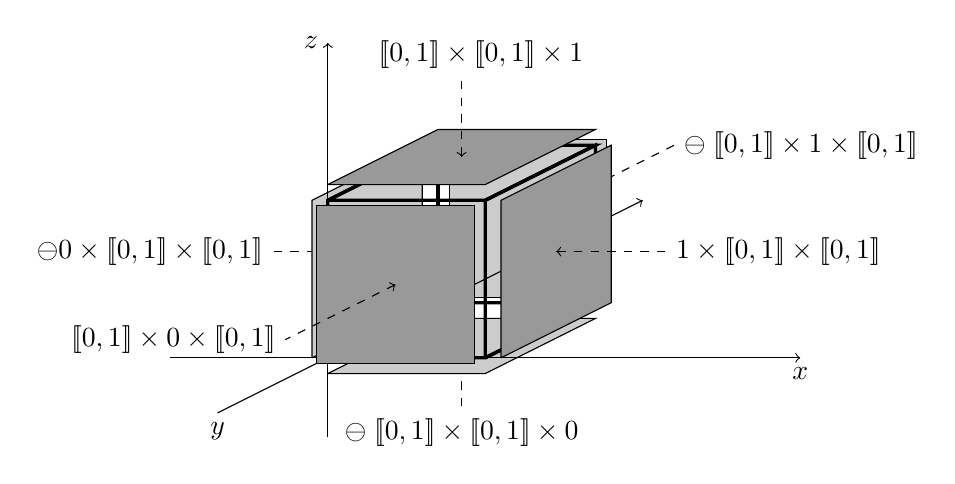
\begin{tikzpicture}[y=1cm, x=2cm]	
	 % back normals
		\draw[color=black, dashed, <-] 
			(0.35, 1.35) --++ 
			(-0.7, 0) node[anchor=east, black] 
			{$\ominus \hset{0} \times [\![0,1]\!] \times [\![0,1]\!]$};
		\draw[color=black, dashed, <-] 
			(1.2,1.7) --++ 
			(1,1) node[anchor=west, black] 
			{$\ominus \; [\![0,1]\!] \times \hset{1} \times [\![0,1]\!]$};
		\draw[color=black, dashed, <-] 
			(0.85,0.35) --++ 
			(0,-1) node[anchor=north, black] 
			{$\ominus \; [\![0,1]\!] \times [\![0,1]\!] \times \hset{0}$};
	 
	 % back faces
	 	\filldraw[fill=black!20] (0,-0.2) --++ (1,0) --++ (0.7,0.7) --++ (-1,0) --++ (-0.7,-0.7);
		\filldraw[fill=black!20] (0.77,0.77) --++ (1,0) --++ (0,2) --++ (-1,0) --++ (0, -2);
		\filldraw[fill=black!20] (-0.1,0) --++ (0,2) --++ (0.7,0.7) --++ (0,-2) --++ (-0.7,-0.7);
	 	
	 % x/y/z axis	
		\draw[->] (-1,0) -- coordinate (x axis mid) (3,0) node[anchor=north] {$x$};
	    	\draw[->] (-0.7,-0.7) node[anchor=north] {$y$} --++ (2.7,2.7) ;
	    	\draw[->] (0,-1) -- coordinate (y axis mid) (0,4) node[anchor=east] {$z$};
		
	% wire frame
		\draw[very thick] (0,0) --++ (1,0) --++ (0.7,0.7) --++ (-1,0) --++ (-0.7,-0.7);
		\draw[very thick] (0.7,0.7) --++ (1,0) --++ (0,2) --++ (-1,0) --++ (0, -2);
		\draw[very thick] (0,0) --++ (0,2) --++ (0.7,0.7) --++ (0,-2) --++ (-0.7,-0.7);
		\draw[very thick] (0,2) --++ (1,0) --++ (0.7,0.7) --++ (-1,0) --++ (-0.7,-0.7);
		\draw[very thick] (0,0) --++ (1,0) --++ (0,2) --++ (-1,0) --++ (0, -2);
		\draw[very thick] (1,0) --++ (0,2) --++ (0.7,0.7) --++ (0,-2) --++ (-0.7,-0.7);
	
	% front faces	
		\filldraw[fill=black!40] (0,2.2) --++ (1,0) --++ (0.7,0.7) --++ (-1,0) --++ (-0.7,-0.7);
		\filldraw[fill=black!40] (-0.07,-0.07) --++ (1,0) --++ (0,2) --++ (-1,0) --++ (0, -2);
		\filldraw[fill=black!40] (1.1,0) --++ (0,2) --++ (0.7,0.7) --++ (0,-2) --++ (-0.7,-0.7);
	
	% front normals
		\draw[color=black, dashed, <-] 
			(1.35+0.1, 1.35) --++ 
			(0.7, 0) node[anchor=west, black] 
			{$\hset{1} \times [\![0,1]\!] \times [\![0,1]\!]$};
		\draw[color=black, dashed, <-] 
			(0.5-0.07,1-0.07) --++ 
			(-0.7,-0.7) node[anchor=east, black] 
			{$[\![0,1]\!] \times \hset{0} \times [\![0,1]\!]$};
		\draw[color=black, dashed, <-] 
			(0.85,2.35+0.2) --++ 
			(0,1) node[anchor=south, black] 
			{$\;\;\;\;\;[\![0,1]\!] \times [\![0,1]\!] \times \hset{1}$};
	\end{tikzpicture}
	\caption[Unit cube with boundary] { 
		The unit cube in $\mathbb{R}^3$ with positive orientation can be represented as the 3-rectangle: 
		$[\![(0,0,0), (1,1,1) ]\!]$ is shown as a wire-frame. 
		The six faces that make up its boundary are shaded and labeled with their corresponding terms.
	\label{fig:cubeboundary} }
\end{figure}

There are several ways to interpret and visualize the $\oplus$ and $\ominus$ sign associated with each face.
Most naturally in $\mathbb{R}^3$ for 2-rectangles is to give each a front and back side with the sign determining which to use.
Alternatively, a 2-rectangle has a boundary formed by 1-rectangles which when drawn as arrows, will all meet head-to-tail.
This induces a clockwise or counter-clockwise cycle around the edge of the rectangle and so $\circlearrowright$ and $\circlearrowleft$ are also commonly used.
This can be seen in Figure \ref{fig:orientation2rect}.
One may even notice that the normals produced by both are the same and choose to use that.
These are all conceptual tools, which are convenient to use particularly in $\mathbb{R}^2$ and $\mathbb{R}^3$.
There may not be such a nice physical interpretation in other spaces.


\begin{figure}[ht] 
	\centering 
	\begin{tikzpicture}
		\def\rectCycle#1#2#3#4{
			\draw[thick, ->, color=black!80] (#1,#2) -- (#3,#2);
			\draw[thick, ->, color=black!60] (#3,#2) -- (#3,#4);
			\draw[thick, ->, color=black!40] (#3, #4) -- (#1,#4);
			\draw[thick, ->, color=black!20] (#1,#4) -- (#1,#2);
			\draw[thick, ->] (#1, 0) -- (#3, 0);
		}
		
		\rectCycle {0+1}{1} {0+2}{2};
		\draw[<->] (0,3) -- (0,0) -- (3,0);
		\draw[very thick, ->] (0,1) -- (0,2);
		\draw (0,1.5) node[anchor=east] {$+$};
		\draw (1.5,0) node[anchor=north] {$+$};
		\draw(1.5,1.5) node {$\;\circlearrowleft^+$};
		  
		\rectCycle {4+2}{1} {4+1}{2};
		\draw[<->] (4+0,3) -- (4+0,0) -- (4+3,0);
		\draw[very thick, ->] (4+0,1) -- (4+0,2);
		\draw (4+0,1.5) node[anchor=east] {$+$};
		\draw (4+1.5,0) node[anchor=north] {$-$};
		\draw(4+1.5,1.5) node {$\;\circlearrowright^-$};
		
		\rectCycle {8+2}{2} {8+1}{1};
		\draw[<->] (8+0,3) -- (8+0,0) -- (8+3,0);
		\draw[very thick, ->] (8+0,2) -- (8+0,1);
		\draw (8+0,1.5) node[anchor=east] {$-$};
		\draw (8+1.5,0) node[anchor=north] {$-$};
		\draw(8+1.5,1.5) node {$\;\circlearrowleft^+$};
		
		\rectCycle {12+1}{2} {12+2}{1};
		\draw[<->] (12+0,3) -- (12+0,0) -- (12+3,0);
		\draw[very thick, ->] (12+0,2) -- (12+0,1);
		\draw (12+0,1.5) node[anchor=east] {$-$};
		\draw (12+1.5,0) node[anchor=north] {$+$};
		\draw(12+1.5,1.5) node {$\;\circlearrowright^-$};
	\end{tikzpicture}
	\caption[Orientations of 2-rectangles] {
		One way of visualizing the orientation of 2-rectangles using clockwise and counter-clockwise cycles 
		of arrows for 1-rectangles. The boundary of $[\![a,b]\!] \times [\![c,d]\!]$ becomes the cycle: 
		$(a,c) \to (b,c) \to (b,d) \to (a,d) \to (a,c)$.
		Showing the relationship between $[\![a,b]\!] \times [\![c,d]\!]$ and $[\![b,a]\!] \times [\![d,c]\!]$ 
	\label{fig:orientation2rect} }
\end{figure}


%%%%%%%%%%%%%%%%%%%%%%%%%%%%%%%%%%%%%%%%%
%
% CHAINS
%
%%%%%%%%%%%%%%%%%%%%%%%%%%%%%%%%%%%%%%%%%
\section{Chains}

In fact, we have already seen $k$-chains without mentioning them explicitly.
The boundary of a $(k+1)$-cube was the sum $\oplus$, of $2(k+1)$, $k$-rectangles.
Chains are not restricted to being boundaries of some larger $(k+1)$ rectangle; 
any linear combination of $k$-rectangles will do.


\begin{definition}
We denote the Abelian group of of all $k$-cubes in $X$ as $C_k(X)$ (omitting $X$ when obvious by context).
An element $c \in C_k$(X) is called a \textbf{$\boldsymbol{k}$-chain on $X$} and is of the form:
\begin{equation*}
	c = \bigoplus_{c_i \in X} \lambda_i c_i
\end{equation*}
with integer coefficients $\lambda_i$ and  $k$-cubes in $c_i$.
If coefficients $\lambda_i$ are $\pm 1$ and $c$ is \emph{locally finite} (i.e. each $c_i$ intersects with only finitely many $c_j$ that have non-zero coefficients) then we say that $c$ is a \textbf{domain of integration}.
\end{definition}


		
Since $k$-chains are just linear combinations of $k$-cubes, we naturally extend many of our definitions linearly as well.
The integral $\int_c f$ of a $k$-chain $c=\bigoplus_i \lambda_i c_i$ is defined as $\lambda_i \int_{c_i} f  + \lambda_2 \int_{c_2} f + \ldots$.
Doing the same for the boundary operator $\partial$ we have:
\begin{align*}
	&\partial_k: C_k \to C_{k-1} \\
	&\partial_k(c) = \bigoplus_{i=1}^k \lambda_i \partial_k(c_i)
\end{align*}
Elegantly, the boundary operator now maps $k$-chains to $(k-1)$-chains!
\begin{equation*}
	\ldots \xleftarrow{\partial_{k-1}} C_{k-1} \xleftarrow{\partial_{k}} C_k \xleftarrow{\partial_{k+1}} C_{k+1} \xleftarrow{\partial_{k+2}} ...
\end{equation*}






%%%%%%%%%%%%%%%%%%%%%%%%%%%%%%%%%%%%%%%%%
% BOUNDARY OF A BOUNDARY
%%%%%%%%%%%%%%%%%%%%%%%%%%%%%%%%%%%%%%%%%
\subsection{Example: \emph{Boundary of a boundary}}

This implies should be able to compute the \emph{boundary of a boundary} of some chain $c \in C_{k+1}$
by composing the boundary function with itself as in:
\begin{equation*}
	\partial_k ( \partial_{k+1} (c)) =\; ?
\end{equation*}
For $c \in C_1$ (i.e $c$ is a 1-rectangle), then $\partial_1(c) \in C_0$ is a set of points.
Since the boundary of any isolated point is empty, $\partial_0$ \emph{always} maps to $\emptyset$. 
So instead let us consider the case when $c \in C_2$ is a 2-rectangle given by: $[\![ a_1 , b_1 ]\!] \times [\![a_2, b_2 ]\!]$
for $a_1 \neq b_1$ and $a_2 \neq b_2$:
\begin{align*}
	\partial_1 ( \partial_2 ( [\![ a_1 , b_1 ]\!] \times [\![a_2, b_2 ]\!] ) )
	=	& 	\; \ominus 	\partial_1( \hset{0} \times [\![0,1]\!]) 
			\; \oplus \; 	\partial_1(\hset{1} \times [\![0,1]\!]) \notag \\
		& 	\; \oplus 	\partial_1( [\![0,1]\!] \times \hset{0}) 
			\; \ominus \; \partial_1([\![0,1]\!] \times \hset{1}) \\
	=	& 	\ominus	( 	\ominus \hset{(0,0)} \oplus \hset{(0,1)} ) 
			\;\oplus\;(	\ominus \hset{(1,0)} \oplus \hset{(1,1)}) \notag \\
		& 	\oplus ( 		\ominus \hset{(0,0)} \oplus \hset{(1,0)} ) 
			\;\ominus\;(	\ominus \hset{(0,1)} \oplus \hset{(1,1)}) \\
	=	& \;\emptyset	
\end{align*}

Geometrically this can be seen below that the boundary of a rectangle are its edges.
The boundary of these edges are the corners; but each corner occurs with both postive and negative sign cancelling.
Often stated as ``$\partial \partial = 0$'', this identity is not unique to $2$-cubes but holds for higher dimensions as well.


\begin{figure}[ht] 
	\centering 
	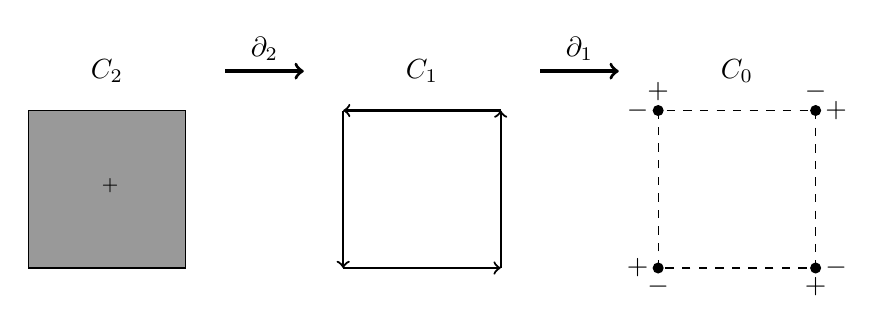
\begin{tikzpicture}[scale=1]
		\draw (1,2.5) node {$C_2$};
		\filldraw[fill=black!40] (0,0) rectangle (2,2);
		\draw (1,1) node {$\;\circlearrowleft^+$};
		
		\draw[very thick, ->] (2.5,2.5) --++ (0.5,0) node[anchor=south] {$\partial_2$} --++ (0.5,0);
		
		\draw (4+1,2.5) node {$C_1$};
		\draw[thick, ->] (4+0,0) --++ (2,0);
		\draw[thick, ->] (4+2,0) --++ (0,2);
		\draw[thick, ->] (4+2,2) --++ (-2,0);
		\draw[thick, ->] (4+0,2) --++ (0,-2);
		
		\draw[very thick, ->] (6.5,2.5) --++ (0.5,0) node[anchor=south] {$\partial_1$} --++ (0.5,0);
		
		\draw (8+1,2.5) node {$C_0$};
		\draw[dashed] (8+0,0) --++ (0,2) --++ (2,0) --++ (0,-2) --++ (-2,0);
		\fill (8,0) node[anchor=north] {$-$} node[anchor=east] {$+$} circle (2pt);
		\fill (8+2,0) node[anchor=west] {$-$} node[anchor=north] {$+$}  circle (2pt);
		\fill (8+2,2) node[anchor=south] {$-$} node[anchor=west] {$+$} circle (2pt);
		\fill (8,2) node[anchor=east] {$-$} node[anchor=south] {$+$} circle (2pt);
	\end{tikzpicture}
	\caption[Boundary of a boundary (of a 2-cube)] {
		The boundary of 2-cube gives a cycle of oriented edges. 
		Taking the boundary of again, at each corner, the negative boundary of one edge 
		will be canceled by the positive boundary of the preceding edge.
	\label{fig:rectboundaryboundary}}
\end{figure}


Let $[\![\boldsymbol{a}, \boldsymbol{b}]\!]$ be a $k$-rectangle in $\mathbb{R}^n$.
Then we have:
\begin{align*}
	\partial_k \partial_{k-1} \left( [\![ \boldsymbol{a}, \boldsymbol{b} ]\!] \right) 
	= \bigoplus_{j=1}^k (-1)^j 
		& \;  \left( \; \partial_{n-1} \left(	
			[\![ 	\boldsymbol{a}^{[\![1,n]\!]}, \;\;
				\boldsymbol{b}^{[\![1,i_j)\!)}
					\oplus \boldsymbol{a}^{[\![i_j]\!]}
					\oplus \boldsymbol{b}^{(\!(i_j,n]\!]} 
			]\!] 
		\right) \right. \notag\\[-1em]
		& \ominus \; \left. \! \partial_{n-1} \left(
			[\![ 	\boldsymbol{a}^{[\![1,i_j)\!)}
					\oplus \boldsymbol{b}^{[\![i_j]\!]}
					\oplus \boldsymbol{a}^{(\!(i_j,n]\!]} , \;\;
				\boldsymbol{b}^{[\![1,n]\!]}
			]\!] 
		\right)\right) \\[1em]
	= \bigoplus_{j=1}^k \bigoplus_{\ell=1}^{k-1} (-1)^{j+\ell}
		\;&
			[\![ 	(\boldsymbol{a}^{[\![1,n]\!]}), \;\;
				(\boldsymbol{b}^{[\![1,i_j)\!) \;\oplus\; (\!(i_j,i_{j,\ell})\!) \;\oplus\; (\!(i_{j,\ell},n]\!]}
					\oplus \boldsymbol{a}^{[\![i_j]\!] \;\oplus\; [\![i_{j,\ell}]\!]})
			]\!] \notag\\[-1em]
		\ominus \;&
			[\![ 	(\boldsymbol{a}^{[\![1,i_{j,\ell})\!) \;\oplus\; (\!(i_{j,\ell},n]\!]}
					\oplus \boldsymbol{b}^{[\![i_{j,\ell}]\!]}), \;\;
				(\boldsymbol{b}^{[\![1,i_j)\!) \;\oplus\; (\!(i_j,n]\!]}
					\oplus \boldsymbol{a}^{[\![i_j]\!]})
			]\!] \notag\\
		\ominus \; &
			[\![ 	(\boldsymbol{a}^{[\![1,i_j)\!) \;\oplus\; (\!(i_j,n]\!]}
					\oplus \boldsymbol{b}^{[\![i_j]\!]}), \;\;
				(\boldsymbol{b}^{[\![1,i_{j,\ell})\!) \;\oplus\; (\!(i_{j,\ell},n]\!]}
					\oplus \boldsymbol{a}^{[\![i_{j,\ell}]\!]})
			]\!] \notag\\
		\oplus \;&
			[\![ 	(\boldsymbol{a}^{[\![1,i_j)\!) \;\oplus\; (\!(i_j,i_{j,\ell})\!) \;\oplus\; (\!(i_{j,\ell},n]\!]}
					\oplus \boldsymbol{b}^{[\![i_j]\!] \;\oplus\; [\![i_{j,\ell}]\!]}), \;\;
				(\boldsymbol{b}^{[\![1,n]\!]})
			]\!] 
\end{align*}
Note that we have $i_j$ and $i'_\ell$; after applying the first boundary operator, one dimension of the $k$-cube is degenerate.
Hence for each sequence: $\{i_j\}_{j=1}^k$ we construct $\{i_{j,\ell}\}_{\ell=1}^{k-1}$ given by:
\begin{equation*}
	i_{j,1} , \ldots, i_{j,k-1} = i_1, \ldots, \widehat{i_j}, \ldots, i_k
\end{equation*}
The double sum iterates over all pairs but $\oplus$ commutes so the $(k-2)$-cube with degenerate dimensions $[\![i_j]\!] \oplus [\![i_{j,\ell}]\!]$ will be iterated over twice. 
The sequences depend on one another so it is not as simple as simply swapping $\ell$ and $j$:
\begin{equation*}
   [\![i_j]\!] \oplus [\![i_{j,\ell}]\!] =
     \begin{cases}
       [\![i_\ell]\!] \oplus [\![i_{\ell,j-1}]\!] & j > \ell \\
       [\![i_{\ell+1}]\!] \oplus [\![i_{\ell+1,j}]\!] & j \leq \ell
     \end{cases}
\end{equation*}


So each term representing a $(k-2)$-cube will occur twice in the sum.
Once with the iteration $(j,\ell)$ and once with $(\ell, j-1)$ or $(\ell+1, j)$.
In either case, $(-1)^{j+\ell}$ is inverted meaning the two cubes will cancel.
Leaving us with the boundary of a boundary being empty.
By linearity this extends to all chains as well as the sum of empty sets is of course still empty.





%%%%%%%%%%%%%%%%%%%%%%%%%%%%%%%%%%%%%%%%%
%
% STOKE'S THEOREM
%
%%%%%%%%%%%%%%%%%%%%%%%%%%%%%%%%%%%%%%%%%
\section{Stokes' Theorem}


This result mirrors the earlier $\diff \diff = 0$ and this duality goes deeper.
The boundary $\partial$ maps a $k+1$-chain to a $k$-chain while 
the exterior derivative $\diff$ mapped a $k$-form to a $k+1$-form.
Sometimes this is written out as:
\begin{equation*}
	\ldots 	\xleftarrow{\partial} C_{k-1} 
			\xleftarrow{\partial} C_k 
			\xleftarrow{\partial} C_{k+1} 
			\xleftarrow{\partial} \ldots
\end{equation*}
\begin{equation*}
	\ldots 	\xrightarrow{\diff} \Lambda^{k-1} 
			\xrightarrow{\diff} \Lambda^k 
			\xrightarrow{\diff} \Lambda^{k+1} 
			\xrightarrow{\diff} \ldots
\end{equation*}
Stokes' Theorem is an important result which links the two even closer and generalizes many classical theorems including
the fundamental theorem of calculus, Green's theorem and the divergence theorem.


Given a $k-1$-form $\omega$ and $k$ chain $M$:
\begin{equation}
	\tag{Stokes' Theorem}
	\int_{\partial M} \omega = \int_M d\omega
\end{equation}


\begin{proof}

First we will consider Stokes theorem for the standard cube $I^k = [0,1]^k \subset \mathbb{R}^k$.
In the previous section we saw how cumbersome representing the faces in $\partial I^k$, could be.
We will denote the faces of $I^k$ by $I^k_{i=0}$ and $I^k_{i=1}$ for the $i$-th faces of $I^k$.
This allows us to rewrite the boundary more succinctly as:
\begin{equation*}
	\partial (I^k) = \bigoplus_{i=1}^k (-1)^i \left( I^k_{i=0} \ominus I^k_{i=1} \right) 
\end{equation*}



A $k-1$-form $\omega$ can be written as the sum
\begin{equation*}
	\omega 
		= \sum_{i=1}^k \omega_i 
		= \sum_{i=1}^k f_i \; \diff x_1 \wedge \ldots \wedge \widehat{\diff x_i} \wedge  \ldots \wedge \diff x_k
\end{equation*}
but since everything: the integrals, $d$ and $\partial$ are all linear, we can work using just one of these terms.
Assuming Stokes' theorem holds for $\omega_i$ then we immediately have it for $\omega$ as well:
\begin{align*}
	\int_{\partial\Omega} \omega 
	&= \int_{\partial \Omega} (\omega_1 + \ldots + \omega_k) \\
	&= \int_{\partial\Omega} \omega_1 + \ldots + \int_{\partial\Omega} \omega_k  \\
	&= \int_{\Omega} d\omega_1 + \ldots + \int_\Omega d\omega_k \\
	&= \int_\Omega (d\omega_1 + \ldots + d\omega_k)\\
	&= \int_\Omega d(\omega_1 + \ldots + \omega_k) = \int_\Omega d\omega
\end{align*}



To compute $d\omega$, we have for each term in the sum:
\begin{align*}
	d \left( f_i \diff x_1 \wedge \ldots \wedge \widehat{\diff x_i} \wedge  \ldots \wedge \diff x_k \right) 
 		&= \diff f_i \wedge \diff x_1 \wedge \ldots \wedge \widehat{\diff x_i} \wedge  \ldots \wedge \diff x_k \\ 
 		&= \left( \sum_{j=1}^k \frac{\partial f_i}{\partial x_j} \diff x_j \right)
 			\wedge \diff x_1 \wedge \ldots \wedge \widehat{\diff x_i} \wedge  \ldots \wedge \diff x_k
\end{align*}
But for $j \neq i$, there will be a duplicate $\diff x_j$ term and this collision will cause the term to go to zero.
Hence only one term in the sum, $i=j$ will actually result in a non-zero term:
\begin{align*}
	\diff \left( f_i \diff x_1 \wedge \ldots \wedge \widehat{\diff x_i} \wedge  \ldots \wedge \diff x_k \right) 
 		&= \left(\frac{\partial f_i}{\partial x_i} \diff x_i \right)
 			\wedge \diff x_1 \wedge \ldots \wedge \hat{\diff x_i} \wedge  \ldots \wedge \diff x_k \\ 
		&= (-1)^{i-1} \frac{\partial f_i}{\partial x_i}
 			 \diff x_1 \wedge \ldots \wedge \diff x_k
\end{align*}



Since this is an integral over the canonical basis $\text{x} = (x_1, \ldots, x_k)$ we can remove the wedge products and
integrate as normal.
\begin{align*}
	\int_{[0,1]^k} \diff \omega_i
		=&\; (-1)^{i-1} \int_{[0,1]^k} \frac{\partial f_i}{\partial x_i}\; \diff(x_1, \ldots, x_k) \\
		=&\; (-1)^{i-1} \int_{[0,1]^{k-1}} \left( \int_0^1 \frac{\partial f_i}{\partial x_i} \diff x_i \right) 
			\diff(x_1, \ldots, \widehat{x_i}, \ldots, x_k)\\
		=&\; (-1)^{i-1}\left( \int_{[0,1]^{k-1}} f_i(x_1, \ldots, x_{i-1}, 1, x_{i+1}, \ldots, x_k)
			\diff(x_1, \ldots, \widehat{x_i}, \ldots, x_k) \right.\\
		&\;	- \left. \int_{[0,1]^{k-1}} f_i(x_1, \ldots, x_{i-1}, 0, x_{i+1}, \ldots, x_k)
			\diff(x_1, \ldots, \widehat{x_i}, \ldots, x_k) \right)
\end{align*}
The trick here being Fubini's Theorem allowing us to evaluate the iterated integral in whichever order we choose.
On the other side of the equality we have:
\begin{align*}
	\int_{\partial I^k} \omega_i
		&= \sum_{j=1}^k (-1)^j \int_{I^k_{j=0}} \omega_i - \int_{I^k_{j=1}} \omega_i
\end{align*}
but $I^k_{j=0}$ is just a $k-1$-rectangle embedded in $\mathbb{R}^k$ by the map:
\begin{equation*}
	(x_1, \ldots x_{k-1}) \mapsto (x_1, \ldots, x_{j-1}, 0, x_{j}, \ldots x_{k-1})
\end{equation*}
So we could alternatively think of $I^k_{j=0}: I^{k-1} \to I^k$ as just a change in coordinates:
\begin{align*}
	\int_{\partial I^k} \omega_i 
		=&\; \sum_{j=1}^k (-1)^j 
			\left(\int_{I^{k-1}} (I^k_{j=0})^*\omega_i - \int_{I^{k-1}} (I^k_{j=1})^* \omega_i \right) \\
		=&\; \sum_{j=1}^k (-1)^j 
			\left(\int_{I^{k-1}} f_i (x_1, \ldots, x_{i-1}, 0, x_{i+1}, \ldots, x_k)
				\diff x_1 \wedge \ldots \wedge \widehat{\diff x_i} \wedge  \ldots \wedge \diff x_k \right. \\
		&	\left. - \int_{I^{k-1}} f_i (x_1, \ldots, x_{i-1}, 1, x_{i+1}, \ldots, x_k)
				\diff x_1 \wedge \ldots \wedge \widehat{\diff x_i} \wedge  \ldots \wedge \diff x_k \right)\\
		=&\; (-1)^i \left(\int_{I^{k-1}} f_i (x_1, \ldots, x_{i-1}, 0, x_{i+1}, \ldots, x_k)
				\diff (x_1, \ldots,\widehat{x_i},  \ldots, x_k) \right. \\
		&	\left. - \int_{I^{k-1}} f_i (x_1, \ldots, x_{i-1}, 1, x_{i+1}, \ldots, x_k)
				\diff (x_1, \ldots,\widehat{x_i},  \ldots, x_k) \right)
\end{align*}



In the final step we observe that all terms in the sum for $i \neq j$ end up disappearing leaving us with just the term for
$i=j$.
Clearly, both sides of the equation are the same and so Stokes' theorem holds for the standard cube.
From here, the remaining cases build on one another are quite straight-forward.
For a singular cube $c$, we have:
\begin{align*}
	\int_{\partial c} \omega
		&= \int_{c (\partial ([0,1]^k))} \omega \\
		&= \int_{\partial( [0,1]^k)} c^* \omega \\
		&= \int_{[0,1]^k} \diff c^* \omega \\
		&= \int_{[0,1]^k} c^* \diff \omega \\
		&= \int_c d\omega
\end{align*}
And for a chain $C=a_1 c_1 + \ldots + a_n c_n$ made up of singular cubes:
\begin{align*}
	\int_C d\omega 
		&= \int_{a_1c_1 + \ldots + a_nc_n	} \diff\omega \\
		&= a_1 \int_{c_1} \diff\omega + \ldots + a_n \int_{c_n} \diff\omega \\
		&= a_1 \int_{\partial c_1} \omega + \ldots + a_n \int_{\partial c_n} \omega \\
		&= \int_{a_1 \partial c_1 + \ldots a_n \partial c_n} \omega \\
		&= \int{\partial ( a_1c_1 + \ldots + a_n c_n)} \omega \\
		&= \int_{\partial C} \omega
\end{align*}

And so we have Stokes' theorem on general chains.
\end{proof}


%%%%%%%%%%%%%%%%%%%%%%%%%%%%%%%%%%%%%%%%%
% CONTOUR EXAMPLE
%%%%%%%%%%%%%%%%%%%%%%%%%%%%%%%%%%%%%%%%%
\subsection{Example: \emph{Contour Integral}}


Generalized partitions can extend past the original domain but so far this has been done through relatively
obvious extensions.
Sometimes the additional regions that are added and negated can be quite unexpected.
\emph{Contour integration} is a method for solving integrals that can involve the usage of curious looking regions to solve.
Consider the following function defined on the real numbers:
\begin{equation*}
	f(x) = \frac{1}{x^4 + 1}
\end{equation*}
and suppose we wish to compute the integral over the entire real line:
\begin{equation*}
	 \int_{-\infty}^\infty f(x) \diff x
\end{equation*}
This is a difficult integral to evaluate directly so instead of treating $f$ as a real function, $f:\mathbb{R} \to \mathbb{R}$, 
we instead consider it as a complex function: $f:\mathbb{C} \to \mathbb{C}$.


Let $C_1$ be the straight line curve from $-r$ to $r$: $C_1(t) =rt-(1-t)r$ and
$C_2$ the circular arc with radius $r$ from $r$  to $-r$: $C_2(t) = re^{it}$.
Finally let $C$ the combined curve: $C= C_1 \oplus C_2$
Then our desired value is the integral over $C_1$ as $r$ goes to infinity:
\begin{equation*}
	\int_{C_1} f(x) \diff x = \oint_{C} f(z) \diff z - \int_{C_2} f(z) \diff z
\end{equation*}


\begin{figure}[ht] 
	\centering 
	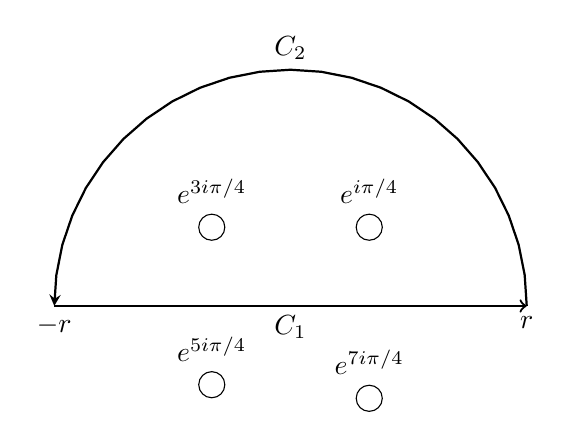
\begin{tikzpicture}
		\draw[>=stealth, thick, ->, domain=0:180] plot ({3*cos(\x)}, {3*sin(\x)});
		\draw[thick, <-] (3,0) node[below] {$r$} -- (-3,0) node[below] {$-r$};
		\node[draw,circle,label=$e^{i \pi/4}$] at (1,1) {};
		\node[draw,circle,label=$e^{3 i \pi/4}$] at (-1,1) {};
		\node[draw,circle,label=$e^{5 i \pi/4}$] at (-1,-1) {};
		\node[draw,circle,below,label=$e^{7 i \pi/4}$] at (1,-1) {};
		\draw (0,3) node[above] {$C_2$};
		\draw (0,0) node[below] {$C_1$};
	\end{tikzpicture}
	\caption[Contour Integral]{
		The contours $C_1$ and $C_2$ and with the four singularities of $f$ marked.
	\label{fig:contourintegration}}
\end{figure}

To solve the integral on $C$ we can use the Cauchy residue theorem: a special case of the generalized Stokes' theorem.
$C$ is a closed simple path and $f$ is holomorphic everywhere except for a finite set of points $\{a_k\}_{i=1}^n$
and so we have:
\begin{equation*}
	\oint_C f(z) \diff z = 2 \pi i \sum_{k=1}^n \Res(f, a_k)
\end{equation*}
And so we must compute the residues of the two singularities above the real line: 
$W_8^1 = e^{i\pi/4}$ and $W_8^3 = e^{3i\pi/4}$.
These are both simple poles and can be computed as follows:
\begin{equation*}
	\Res(f, W_8^1) =\lim_{z \to W_8^1} \frac{z - W_8^1}{z^4 +1} 
		= \lim_{z \to W_8^1} \frac{1}{4z^3}
		= (1/4) W_8^{-3} = (1/4) W_8^5
\end{equation*}
\begin{equation*}
	\Res(f, W_8^3) =\lim_{z \to W_8^3} \frac{z - W_8^3}{z^4 +1} 
		= \lim_{z \to W_8^3} \frac{1}{4z^3}
		= (1/4) W_8^{-9} = (1/4) W_8^7
\end{equation*}
Converting these out of polar coordinates, we have 
	$W_8^7 = \left( \frac{\sqrt{2}}{2}-\frac{\sqrt{2}}{2}i \right)$ 
	and $W_8^5 =\left( -\frac{\sqrt{2}}{2}-\frac{\sqrt{2}}{2}i \right)$:
\begin{equation*}
	\oint_C f(z) \diff z 
	= 2 \pi i \left( 	\frac{1}{4} \left( \frac{\sqrt{2}}{2}-\frac{\sqrt{2}}{2}i \right) 
				+	\frac{1}{4} \left( -\frac{\sqrt{2}}{2}-\frac{\sqrt{2}}{2}i \right)\right)
	= \frac{\pi}{\sqrt{2}}
\end{equation*}
To compute the integral over $C_2$, we make the substitutions, $z = re^{i \theta}$ and $dz=ire^{i\theta} d\theta$:
\begin{equation*}
	\int_{C_2} f(z) \diff z = \int_0^\pi \frac{ire^{i\theta}}{r^4 e^{4i\theta} +1} \diff\theta
\end{equation*}
And then simply observe that as $r$ goes to infinity, this integral goes to zero and the term for $C_2$ drops off.
Leaving us with just:
\begin{equation*}
	\int_{-\infty}^\infty f(x) \diff x = \frac{\pi }{\sqrt{2}}
\end{equation*}